\documentclass[10pt]{article}
\usepackage[polish]{babel}
\usepackage[utf8]{inputenc}
\usepackage[T1]{fontenc}
\usepackage{amsmath}
\usepackage{amsfonts}
\usepackage{amssymb}
\usepackage[version=4]{mhchem}
\usepackage{stmaryrd}
\usepackage{graphicx}
\usepackage[export]{adjustbox}
\graphicspath{ {./images/} }

\title{GIMNAZJUM }

\author{}
\date{}


\begin{document}
\maketitle
\begin{enumerate}
  \item Dany jest trójkąt \(A B C\), w którym \(A B=10, A C=B C=20\). Obliczyć długość odcinka łączącego punkty styczności okręgu wpisanego w ten trójkąt do boków \(A C\) i \(B C\).
  \item Z punktu \(P\) leżącego na zewnątrz okręgu poprowadzono styczną do okręgu w punkcie \(A\) i sieczną przecinającą okrąg w punktach \(B\) i \(C\). Udowodnij, że
\end{enumerate}

\[
P A^{2}=P B \cdot P C
\]

\begin{enumerate}
  \setcounter{enumi}{2}
  \item Dany jest czworokąt wypukły \(A B C D\). Punkt P jest punktem\\
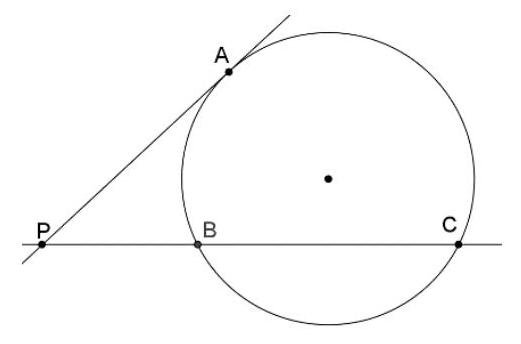
\includegraphics[max width=\textwidth, center]{2024_11_21_e38482f605918448c267g-1}\\
przecięcia przekątnych tego czworokąta. Udowodnij, że jeżeli \(P A \cdot P C=P B \cdot P D\), to na czworokącie \(A B C D\) można opisać okrąg.
\end{enumerate}

\section*{LICEUM}
\begin{enumerate}
  \item Dany jest trapez \(A B C D\) o polu 15 i podstawach \(A B\) i \(C D\). Dwusieczna kąta \(A B C\) jest prostopadła do ramienia \(A D\) i przecina je w takim punkcie E, że \(\frac{A E}{E D}=2\). Obliczyć pola figur \(A B E\) i \(E B C D\), na które został podzielony trapez.
  \item Dany jest czworokąt wypukły \(A B C D\) nie będący trapezem. Punkt \(P\) jest punktem przecięcia prostych \(A D\) i \(B C\). Udowodnij, że jeżeli \(P A \cdot P D=P B \cdot P C\), to na czworokącie \(A B C D\) można opisać okrąg.
  \item W trójkącie ostrokątnym \(A B C\) wysokość poprowadzona z wierzchołka \(A\) przecina okrąg o średnicy \(B C\) w punktach \(K\) i \(L\), a wysokość poprowadzona z wierzchołka \(B\) przecina okrąg o średnicy \(A C\) w punktach \(M\) i \(N\). Udowodnij, że na czworokącie KMLN można opisać okrąg.\\
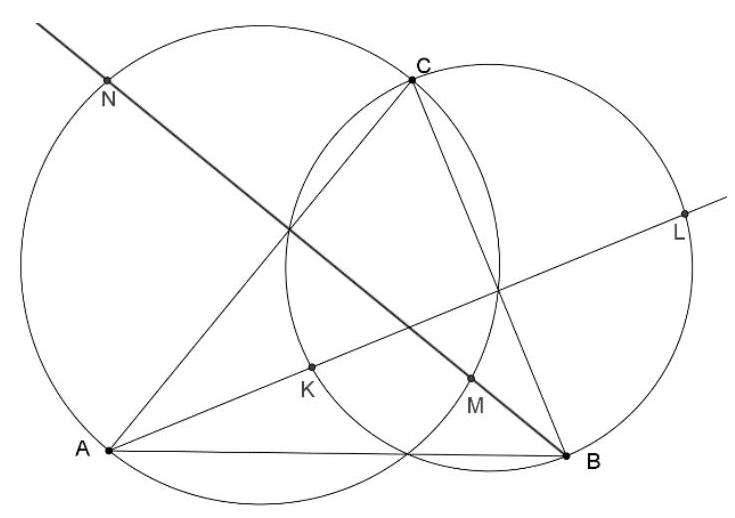
\includegraphics[max width=\textwidth, center]{2024_11_21_e38482f605918448c267g-1(1)}
\end{enumerate}

\end{document}